% This file was created by tikzplotlib vunknown.
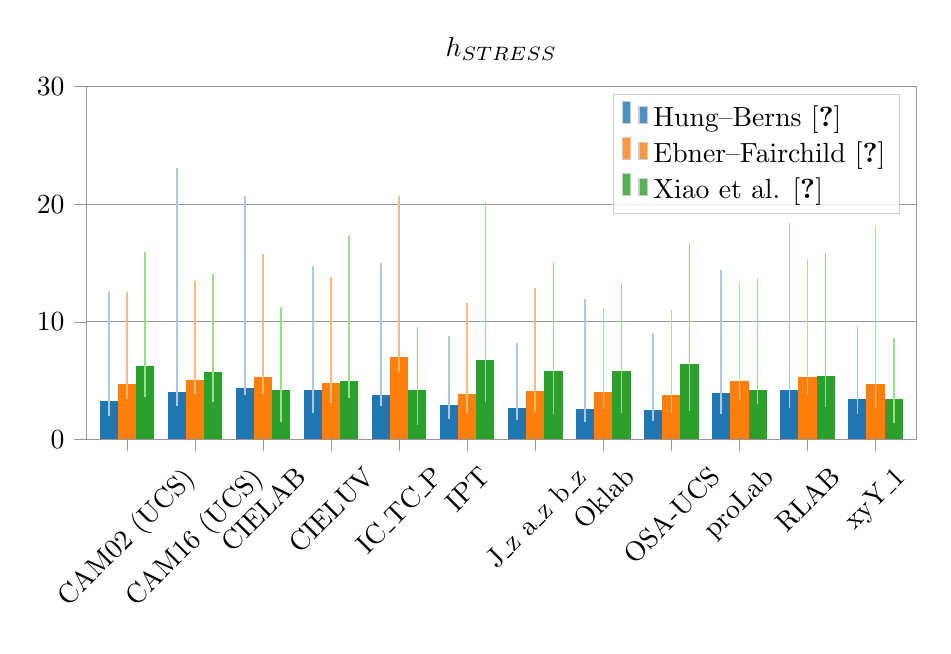
\begin{tikzpicture}

\definecolor{color0}{rgb}{0.682352941176471,0.780392156862745,0.909803921568627}
\definecolor{color1}{rgb}{1,0.733333333333333,0.470588235294118}
\definecolor{color2}{rgb}{0.596078431372549,0.874509803921569,0.541176470588235}
\definecolor{color3}{rgb}{0.12156862745098,0.466666666666667,0.705882352941177}
\definecolor{color4}{rgb}{1,0.498039215686275,0.0549019607843137}
\definecolor{color5}{rgb}{0.172549019607843,0.627450980392157,0.172549019607843}

\begin{axis}[
axis line style={white!58.8235294117647!black},
height=0.5\textwidth,
legend cell align={left},
legend style={fill opacity=0.8, draw opacity=1, text opacity=1, draw=white!80!black},
tick align=outside,
tick pos=left,
title={\(\displaystyle h_{STRESS}\)},
width=\textwidth,
x grid style={white!58.8235294117647!black},
xmin=-0.6, xmax=11.6,
xtick style={color=white!58.8235294117647!black},
xtick={0,1,2,3,4,5,6,7,8,9,10,11},
xticklabel style = {rotate=45.0},
xticklabels={CAM02 (UCS),CAM16 (UCS),CIELAB,CIELUV,IC\_TC\_P,IPT,J\_z a\_z b\_z,Oklab,OSA-UCS,proLab,RLAB,xyY\_1},
y grid style={white!58.8235294117647!black},
ymajorgrids,
ymin=0, ymax=30,
ytick style={color=white!58.8235294117647!black}
]
\draw[draw=none,fill=color3] (axis cs:-0.4,0) rectangle (axis cs:-0.133333333333333,3.26752096358108);
\addlegendimage{ybar,ybar legend,draw=none,fill=color3};
\addlegendentry{Hung--Berns \cite{hung}}

\draw[draw=none,fill=color3] (axis cs:0.6,0) rectangle (axis cs:0.866666666666667,4.03663610711869);
\draw[draw=none,fill=color3] (axis cs:1.6,0) rectangle (axis cs:1.86666666666667,4.34856818798823);
\draw[draw=none,fill=color3] (axis cs:2.6,0) rectangle (axis cs:2.86666666666667,4.21626028738579);
\draw[draw=none,fill=color3] (axis cs:3.6,0) rectangle (axis cs:3.86666666666667,3.79577398935562);
\draw[draw=none,fill=color3] (axis cs:4.6,0) rectangle (axis cs:4.86666666666667,2.92119683105357);
\draw[draw=none,fill=color3] (axis cs:5.6,0) rectangle (axis cs:5.86666666666667,2.68536426894408);
\draw[draw=none,fill=color3] (axis cs:6.6,0) rectangle (axis cs:6.86666666666667,2.63371950519244);
\draw[draw=none,fill=color3] (axis cs:7.6,0) rectangle (axis cs:7.86666666666667,2.49530998013144);
\draw[draw=none,fill=color3] (axis cs:8.6,0) rectangle (axis cs:8.86666666666667,3.98758591406573);
\draw[draw=none,fill=color3] (axis cs:9.6,0) rectangle (axis cs:9.86666666666667,4.2018217479834);
\draw[draw=none,fill=color3] (axis cs:10.6,0) rectangle (axis cs:10.8666666666667,3.44018748653443);
\draw[draw=none,fill=color4] (axis cs:-0.133333333333333,0) rectangle (axis cs:0.133333333333333,4.75235322590401);
\addlegendimage{ybar,ybar legend,draw=none,fill=color4};
\addlegendentry{Ebner--Fairchild \cite{ebner}}

\draw[draw=none,fill=color4] (axis cs:0.866666666666667,0) rectangle (axis cs:1.13333333333333,5.07600805665884);
\draw[draw=none,fill=color4] (axis cs:1.86666666666667,0) rectangle (axis cs:2.13333333333333,5.30715095336481);
\draw[draw=none,fill=color4] (axis cs:2.86666666666667,0) rectangle (axis cs:3.13333333333333,4.82895376092783);
\draw[draw=none,fill=color4] (axis cs:3.86666666666667,0) rectangle (axis cs:4.13333333333333,7.04859738515829);
\draw[draw=none,fill=color4] (axis cs:4.86666666666667,0) rectangle (axis cs:5.13333333333333,3.8585452834895);
\draw[draw=none,fill=color4] (axis cs:5.86666666666667,0) rectangle (axis cs:6.13333333333333,4.11463844120849);
\draw[draw=none,fill=color4] (axis cs:6.86666666666667,0) rectangle (axis cs:7.13333333333333,4.05730886560146);
\draw[draw=none,fill=color4] (axis cs:7.86666666666667,0) rectangle (axis cs:8.13333333333333,3.81297237590754);
\draw[draw=none,fill=color4] (axis cs:8.86666666666667,0) rectangle (axis cs:9.13333333333333,4.94612094628322);
\draw[draw=none,fill=color4] (axis cs:9.86666666666667,0) rectangle (axis cs:10.1333333333333,5.35024616302759);
\draw[draw=none,fill=color4] (axis cs:10.8666666666667,0) rectangle (axis cs:11.1333333333333,4.75045818919245);
\draw[draw=none,fill=color5] (axis cs:0.133333333333333,0) rectangle (axis cs:0.4,6.20819583068422);
\addlegendimage{ybar,ybar legend,draw=none,fill=color5};
\addlegendentry{Xiao et al. \cite{xiao}}

\draw[draw=none,fill=color5] (axis cs:1.13333333333333,0) rectangle (axis cs:1.4,5.72257615772014);
\draw[draw=none,fill=color5] (axis cs:2.13333333333333,0) rectangle (axis cs:2.4,4.23955931207377);
\draw[draw=none,fill=color5] (axis cs:3.13333333333333,0) rectangle (axis cs:3.4,4.94778942179497);
\draw[draw=none,fill=color5] (axis cs:4.13333333333333,0) rectangle (axis cs:4.4,4.16705224310066);
\draw[draw=none,fill=color5] (axis cs:5.13333333333333,0) rectangle (axis cs:5.4,6.77347388639463);
\draw[draw=none,fill=color5] (axis cs:6.13333333333333,0) rectangle (axis cs:6.4,5.79350009458331);
\draw[draw=none,fill=color5] (axis cs:7.13333333333333,0) rectangle (axis cs:7.4,5.83206308550637);
\draw[draw=none,fill=color5] (axis cs:8.13333333333333,0) rectangle (axis cs:8.4,6.37866193244546);
\draw[draw=none,fill=color5] (axis cs:9.13333333333333,0) rectangle (axis cs:9.4,4.20192601604066);
\draw[draw=none,fill=color5] (axis cs:10.1333333333333,0) rectangle (axis cs:10.4,5.38373889554074);
\draw[draw=none,fill=color5] (axis cs:11.1333333333333,0) rectangle (axis cs:11.4,3.40752186432333);
\path [draw=color0, semithick]
(axis cs:-0.266666666666667,2.01344106609042)
--(axis cs:-0.266666666666667,12.585831162163);

\path [draw=color0, semithick]
(axis cs:0.733333333333333,2.88204238274443)
--(axis cs:0.733333333333333,23.0821251838036);

\path [draw=color0, semithick]
(axis cs:1.73333333333333,3.74220236663768)
--(axis cs:1.73333333333333,20.6838582951699);

\path [draw=color0, semithick]
(axis cs:2.73333333333333,2.24044577432782)
--(axis cs:2.73333333333333,14.7383255154587);

\path [draw=color0, semithick]
(axis cs:3.73333333333333,2.87068598460373)
--(axis cs:3.73333333333333,14.9848570240094);

\path [draw=color0, semithick]
(axis cs:4.73333333333333,1.72693435192158)
--(axis cs:4.73333333333333,8.81598126109674);

\path [draw=color0, semithick]
(axis cs:5.73333333333333,1.67603753091287)
--(axis cs:5.73333333333333,8.24506868541112);

\path [draw=color0, semithick]
(axis cs:6.73333333333333,1.51635225412582)
--(axis cs:6.73333333333333,11.9536972847795);

\path [draw=color0, semithick]
(axis cs:7.73333333333333,1.53981557412956)
--(axis cs:7.73333333333333,9.08762942974483);

\path [draw=color0, semithick]
(axis cs:8.73333333333333,2.19325999358212)
--(axis cs:8.73333333333333,14.4085853507735);

\path [draw=color0, semithick]
(axis cs:9.73333333333333,2.69883014342922)
--(axis cs:9.73333333333333,18.4482886967338);

\path [draw=color0, semithick]
(axis cs:10.7333333333333,2.12892068183501)
--(axis cs:10.7333333333333,9.62735767650436);

\path [draw=color1, semithick]
(axis cs:0,3.424998465871)
--(axis cs:0,12.5071317722814);

\path [draw=color1, semithick]
(axis cs:1,3.88874750268467)
--(axis cs:1,13.4370631564062);

\path [draw=color1, semithick]
(axis cs:2,3.88316164215114)
--(axis cs:2,15.7533478737416);

\path [draw=color1, semithick]
(axis cs:3,3.07017097519348)
--(axis cs:3,13.7984716412401);

\path [draw=color1, semithick]
(axis cs:4,5.75659406786079)
--(axis cs:4,20.676646161224);

\path [draw=color1, semithick]
(axis cs:5,2.24526276016063)
--(axis cs:5,11.5808848549903);

\path [draw=color1, semithick]
(axis cs:6,2.33397236461023)
--(axis cs:6,12.9201965254808);

\path [draw=color1, semithick]
(axis cs:7,2.56130471254741)
--(axis cs:7,11.2190267888432);

\path [draw=color1, semithick]
(axis cs:8,2.26308901563546)
--(axis cs:8,10.9915837067322);

\path [draw=color1, semithick]
(axis cs:9,3.36957663808249)
--(axis cs:9,13.3981922557017);

\path [draw=color1, semithick]
(axis cs:10,3.75636388767855)
--(axis cs:10,15.313118958246);

\path [draw=color1, semithick]
(axis cs:11,2.68628272719787)
--(axis cs:11,18.18594988029);

\path [draw=color2, semithick]
(axis cs:0.266666666666667,3.63894467133903)
--(axis cs:0.266666666666667,15.9510200449838);

\path [draw=color2, semithick]
(axis cs:1.26666666666667,3.16028905713057)
--(axis cs:1.26666666666667,14.0654559704759);

\path [draw=color2, semithick]
(axis cs:2.26666666666667,1.47502195501124)
--(axis cs:2.26666666666667,11.2261300003756);

\path [draw=color2, semithick]
(axis cs:3.26666666666667,3.54855537687839)
--(axis cs:3.26666666666667,17.3790745169416);

\path [draw=color2, semithick]
(axis cs:4.26666666666667,1.20599891619739)
--(axis cs:4.26666666666667,9.52255164752983);

\path [draw=color2, semithick]
(axis cs:5.26666666666667,3.20391234458793)
--(axis cs:5.26666666666667,20.1607173258571);

\path [draw=color2, semithick]
(axis cs:6.26666666666667,2.13932444531394)
--(axis cs:6.26666666666667,15.0853390244697);

\path [draw=color2, semithick]
(axis cs:7.26666666666667,2.27697561512914)
--(axis cs:7.26666666666667,13.3000312805048);

\path [draw=color2, semithick]
(axis cs:8.26666666666667,2.43116442514678)
--(axis cs:8.26666666666667,16.6933620755534);

\path [draw=color2, semithick]
(axis cs:9.26666666666667,2.98907849016281)
--(axis cs:9.26666666666667,13.7320281149822);

\path [draw=color2, semithick]
(axis cs:10.2666666666667,2.7933451374924)
--(axis cs:10.2666666666667,15.819379668067);

\path [draw=color2, semithick]
(axis cs:11.2666666666667,1.39017099986293)
--(axis cs:11.2666666666667,8.67083273052145);

\end{axis}

\end{tikzpicture}
